%FEBRUARY 2020, made by the TeXniCie with some code copied from Freek Geerligs' bachelor thesis presentation
% minor adjustments made in March 2023 by the TeXniCie

\documentclass{beamer}

% Packages:
%\usepackage[a4paper]{geometry} 
\usepackage[english]{babel} 	% correct linebreaks etc.
\usepackage{%
	parskip, 					% alinea's (no indent, whitespace)
	amsmath, amssymb,			%
	textcomp,amsthm, 			% Mathematical symbols etc.
	color, 						% Colors
	enumerate,					% For enumerations
	hyperref,					% clickable links in pdf
	graphicx,					% For including pictures
	caption,
	%subcaption,
	%subfig,
	mathrsfs,
	amsthm, 					% Definition,proof,... environments		
	tikz-cd						% For commutative diagrams
}

%%%%%%%%%%%%%%%%%%%%%%%%%%%%%%%%%%%%%

% Below layout for definitions and proof related things
\theoremstyle{definition}
\newtheorem{dfn}{Definition}[section]% nummering van definities volgt nu met secties
\theoremstyle{example}
\newtheorem{conseq}[dfn]{Consequence}
\newtheorem{const}[dfn]{Construction}
%\theoremstyle{plain}
\newtheorem{thm}[dfn]{Stelling}% nummering van stellingen loopt nu samen met dfn (als [dfn] aan het eind zou staan, zou het een nieuw getal erachter betekenen)
%\newtheorem{lemma}[dfn]{Lemma}
%\newtheorem{example}[]{Example}
%\newtheorem{nexample}[example]{Non-example}

%%%%%%%%%%%%%%%%%%%%%%%%%%%%%%%%%%%%%%%%%

% Layout for the presentation (colours etc.), a-eskwadraat has its own theme, but you can choose another theme. (Highly recommended for a bit more professionality.)

\usetheme{aes2}
%\usetheme{Frankfurt} % Another similar theme without the a-es logo
%\usecolortheme{dolphin} %crane or dolphin are nice
%\useinnertheme{circles}
%\useoutertheme{smoothbars}

%%%%%%%%%%%%%%%%%%%%%%%%%%
% Modify these for your own presentation.
\title{Title of your presentation}
\date{Your presentation date, for example \today}
\author{Your name here}

\begin{document}
	
	\begin{frame}
		\titlepage
	\end{frame}	
	
	\begin{frame}{Content}% each slide (with name between {} ) is in the frame-environment
		\tableofcontents
	\end{frame}
	
	\section{First subject}
	% The structure (sections, subsections etc.) like you're used to in TeX-files also work in the beamer class, it affects the progress part of the slides (at the top).	
	
	\begin{frame}
		\frametitle{What you should know before I start with my thesis work}
		In the frame-environment you can do what you're used to to make it print on a slide. For example use text and formula's like
		\begin{align}
			E &= \frac{p^2}{2m}\\
			E_{rel}^2 &= m^2c^4 + p^2c^2
		\end{align}
		\begin{block}{Important}
			It is very   I M P O R T A N T   to be able to \emph{emphasise} in \textit{different} \textbf{ways}!
		\end{block}
	\end{frame}


\begin{frame}{Let's continue}
Sometimes it is a shame if everything you want to say is already on the slide.\newline
\begin{thm}
	You do not yet know the proof of this theorem.
\end{thm}
\begin{block}{Proof}
	The proof is here.
\end{block}
But we can fix this!

Let's try this again.

\end{frame}

\subsection{This subsection is not in the progress bar but is in the table of contents!}

\begin{frame}{Again!}
\begin{thm}
	You do not yet know the proof of this theorem.
\end{thm}
\pause
\begin{block}{Proof}
	The proof is here.
\end{block}
\pause
Much better!
\end{frame}

\begin{frame}{More advanced}
	\only<1->{We can even make the text disappear. (Or keep an important text/formula on your slide.)\\}
	\only<2-3>{Peekaboo!\\}
	\only<3>{Go and seek! (by lack of a better translation of \textit{Wie niet weg is is gezien!})}
	\only<4>{And let's go on...}
\end{frame}

\begin{frame}
Enumerations can look better this way as well
\begin{itemize}
	\only<1-2>{\item 1...}
	\only<2-3>{\item 2...}
	\only<3-4>{\item 3...}
	\only<4-5>{\item 4, 5, 6, 7, 8}
	\only<5-6>{\item 9...}
	\only<6>{\item 10!}
	\only<7>{\item Ready or not here I come!}
\end{itemize}

\end{frame}

%\begin{frame}{Even more advanced, taken from a thesis presentation}
%
%\begin{columns}[T] % align columns
%	\uncover<6->{	\begin{column}{.48\textwidth}
%			\begin{dfn}
%				For $x,y\in \hat R$, we define 
%				the \textbf{Kuratowski-tuple } $(x,y)$ as
%				$$(x,y):=\big\{\{x\},\{x,y\}\big\}$$ 
%			\end{dfn}
%	\end{column}}%
%	
%	\begin{column}{.48\textwidth}
%		
%	\begin{block}{The superstructure}
%	\begin{itemize}
%		\item			$R_0:=\mathbb R$. 
%		\item			$R_{n+1}:=\mathcal P(\bigcup\limits_{k=0}^nR_{k}),$ 
%		\item			$\hat R:= \bigcup\limits_{n\in\mathbb N} R_n$.
%	\end{itemize}
%\end{block}
%	\end{column}%
%	\hfill%
%
%
%\end{columns}
%\pause
%\begin{align*}
%	\uncover<3->{0,1,2 & \in }R_0	=\mathbb R
%	\\
%\uncover<4->{	\mathbb N, \mathbb Z, \mathbb Q, \mathbb R,\{0\},\{0,1\}&\in }R_1	=\mathcal P(\mathbb R)
%	\\ 
%\uncover<5->	{\mathcal T_{eucl}, \big\{\{0\},\{0,1\}\big\}&\in} R_2 =\mathcal P(\mathbb R\cup \mathcal P(\mathbb R))
%	\\
%\uncover<7->	{   \mathbb R^2, \{(x,x+1)|x\in\mathbb R \}, \{(x,y)|x\leq y\}&\in }R_3 =\mathcal P(R_0\cup R_1\cup R_2)
%\\
%\uncover<8->	{  C^\infty(\mathbb R), \mathbb R^\mathbb R, \mathbb R^\mathbb N&\in }R_4 =\mathcal P(R_0\cup R_1\cup R_2\cup R_3)\end{align*}
%
%
%\end{frame}

\section{Applications}

\begin{frame}
\begin{columns}[T]
	\begin{column}[T]{5cm}
		We can also place colums next to each other.
		
		\begin{block}{Also cool}
			More indents in your code.
		\end{block}
		\begin{alertblock}{Attention!}
			A block for even more \emph{emphasis}!
			
			Just differently colored.
		\end{alertblock}
	\end{column}
	\begin{column}[T]{5cm}
		We can even include pictures!
		\begin{figure}
			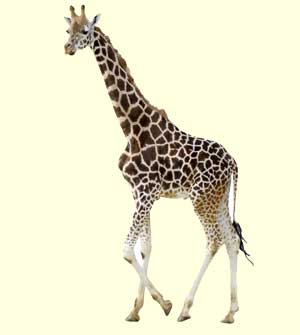
\includegraphics[scale=0.4]{Giraffe_klein.jpg}
			\caption{A picture you might recognise.}
		\end{figure}
		
	\end{column}
\end{columns}
\end{frame}


\section{Also}


\begin{frame}{Also}
Don't forget to compile, the table of contents and the progress bar will need more than one compilation to be updated correctly.

At the end of a presentation you thank your audience and leave room for questions.

Then your presentation is done!
\end{frame}


\begin{frame}{P.S.}
	It looks a bit more professional not to have the a-eswiggle on each slide.
	How to remove this is in the code. %see the layout section of the preamble.
\end{frame}

\end{document}